There are many studies that focus on applying computer vision to fencing. For example, Takahashi\cite{takahashi2020real} et al. proposed a robust detection and tracking method to visualize the trajectory of a fencing sword for live TV programs. Since live TV programs require not only accuracy but also real-time computation, they successfully track fast-moving fencing swords by using supervised machine learning to detect the swords and using a particle filter to predict their positions in the next frame.

Athow\cite{athowusing} et al. proposed a computer vision-based scoring system to assist referees in foil events in fencing. They used color blob detection to track fencers who wore color patches on their hands.

In addition, there have been cases of computer vision and motion analysis: Makawaski et al. \cite{MALAWSKI20181} created a new local trace image to represent fencing motions, and showed that the dynamics of the motion is useful for analyzing similar motion patterns. They showed that motion dynamics can be useful for analyzing similar motion patterns. In the same study, he also created a dataset for analyzing footwork, contributing to the development of the field.

However, there is still no research that proposes a comprehensive framework for extracting posture and positional information from video in fencing and performing tactical analysis to gain an advantage in competition.

In this study, we propose an analysis framework that uses computer vision and machine learning to extract posture and position information to assist experts in their analysis tasks.

\begin{figure}[!htbp]
    \centering
	\begin{tabular}{c}
		\subfloat[Broadcast images of sword trajectories at All Japan Fencing Championship 2017]
            {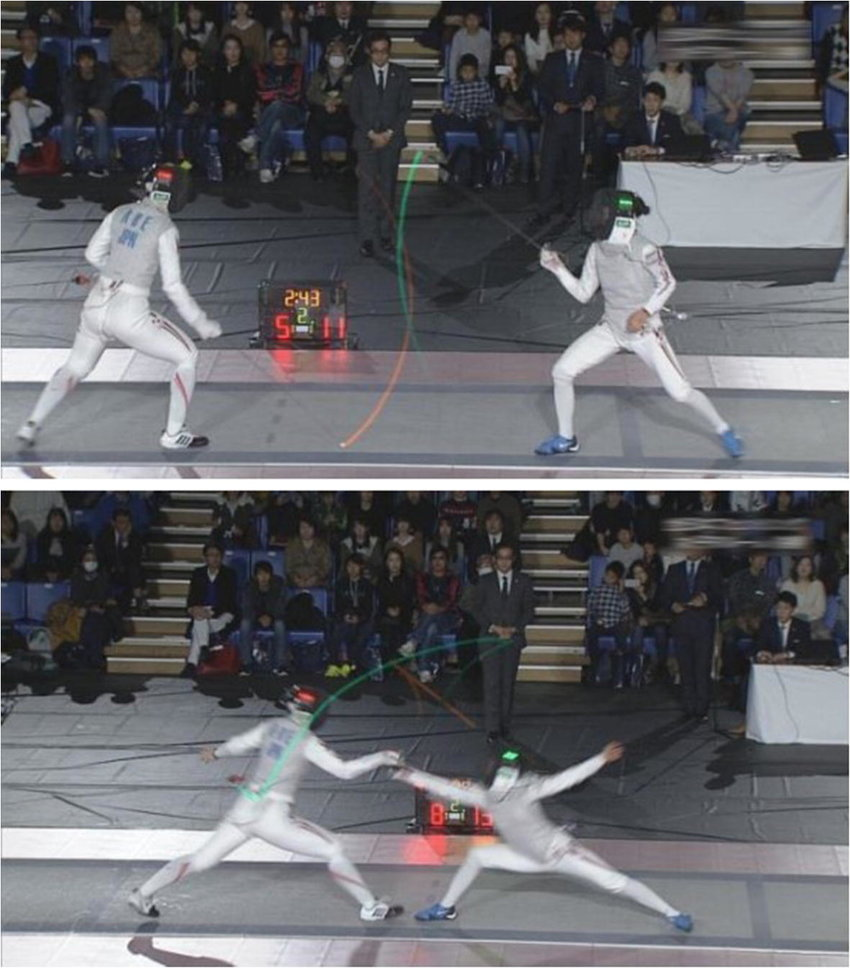
\includegraphics[width=0.5\textwidth]{images/fencing/pw-1.png}} \\
		\subfloat[Photos of the RGB/IR camera]
            {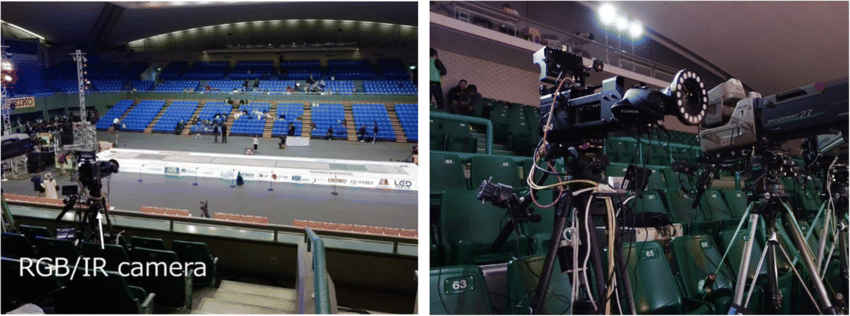
\includegraphics[width=0.5\textwidth]{images/fencing/pw-2.png}} \\                                             \\
		\subfloat[Photos of equipment in operations area]
            {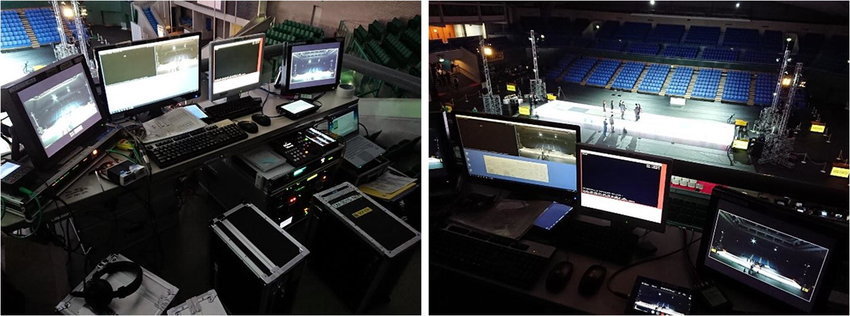
\includegraphics[width=0.5\textwidth]{images/fencing/pw-3.png}}
	\end{tabular}
	\caption{Images of study conducted in \cite{takahashi2020real}}
\end{figure}
